\chapter{Methodology and experiment}

\section{Web-application}
This thesis used an online web-based survey to conduct the experiment. An online survey avoid the cost and effort of printing, distributing, and collecting paper forms. Many people prefer to answer a brief survey displayed on a screen instead of filling in and returning a printed form \citep{Ben2009}.   

In a self selected sample, which is some the case here, there is potentially a bias in the sample \citep{Ben2009}. %s168

\section{Pilot test}
It is important to pilot test the survey prior to actual use \citep{Ben2009}. A pilot test provides an opportunity to validate the wording of the tasks, do the participants understand the tasks? It also helps understand the time necessary for completing the survey, which should be communicated to the participants in prior to the survey \citep{Schade2015}. The pilot-test is conducted with a small sample of users. Results from the pilot-test can be used to determine the sample size. The sample size tells us how many responses that are needed \citep{Smith2013}. The formula for determining the sample size requires the standard deviation, how much variance to expect in the response \citep{Smith2013}. This standard deviation can be calculated from the pilot-test results.

A pilot test was conducted with a total of eight participants, five experienced and three non-experienced participants aged from 22 to 64 years. After the pilot test the usability was measured. The standard ISO 9241-11 suggests that measures of usability should cover effectiveness, efficiency and satisfaction \citep{ISO1998}. Measuring these three classes of metric can vary widely and makes it difficult to make comparisons of usability between different systems. " just because a particular design feature has proved to be very useful in making one system usable does not necessarily mean that it will do so for another system" \citep{Brooke1996}. Usability in this thesis was measures with the \textit{System Usability Scale}(SUS). This scale gives an subjective measure of usability and was developed by John Brooke. The \textit{System Usability Scale} questionnaire consists of ten statements where the participants rate their agreement in an five-point scale \citep{Ben2009}. Subjective measure of usability is usually obtained through the use of questionnaire and attitude scales \citep{Brooke1996}. SUS was developed to be quick and simple, but also reliable enough to be able to compare performance changes between versions \citep{Brooke1996}.  

The usability is important to measure. If the participants doesn't understand how the web-application works, they will probably not do the survey since they then have to invest time in understanding what to do. %they will either exit the survey or answer the questions in the survey wrong. 
Usability is an important factor to get enough participants to do the whole survey and not quit halfway. 

\subsection{Execution of the pilot test}
The pilot test started with a brief information about this study and the survey. They where told to talk out load during the survey, no help or guidance was given to the participants. The author observed the participants while they conducted the survey. The author took notes and watched if the participants understood the questions in the survey correctly. After the survey a \textit{System Usability Scale} questionnaire was answered by the participants. At the end the participants was asked to give general feedback on the web-application. The SUS score and the feedback was then used to determine the usability of the web-application and to determine which improvements to be done.  

\subsection{Results from the pilot test}

- Did someone knew micro-tasking? Can we see something here?

The average SUS score was 84.64 out of 100. 

All participants thought that the instruction movie was confusing. It was short, the instructions went too fast and it lacked voice descriptions. The movie needed major improvements. 

Overall feedback on the tasks was that it was difficult to understand which building was which and also if the building shape layer was selected or not in question one. The lack of labels on the building was done on purpose to get the task as much as possible realistic. The selection of best fitting shape needed improvements, it had to be made clearer that selection was done by clicking on the shape, not by using the layer control as some thought. 
 
Also, some pages had too much information and long sentences. The task progress bar was removed, no one noticed it, only the survey progress bar on the top right is necessary. 

The two oldest participants spent almost twice as much time on the test than the younger. Maybe it where too much cognitive load on them. Learning a new application and at the same time understanding how to do the survey and answer the questions given to them. One of them where experienced and the other non-experienced, so this is a surprising result.  CHECK THE TIME ON EACH TASK FOR THE OLDER PARTICIPANTS. Figure \ref{fig:allparticipantssortedageparticipantexclude4notitle} show the task results from all participants ordered by age. There are three entries per participant, so three and three bars are results from the same participant. 

\begin{figure}[h]
	\centering
	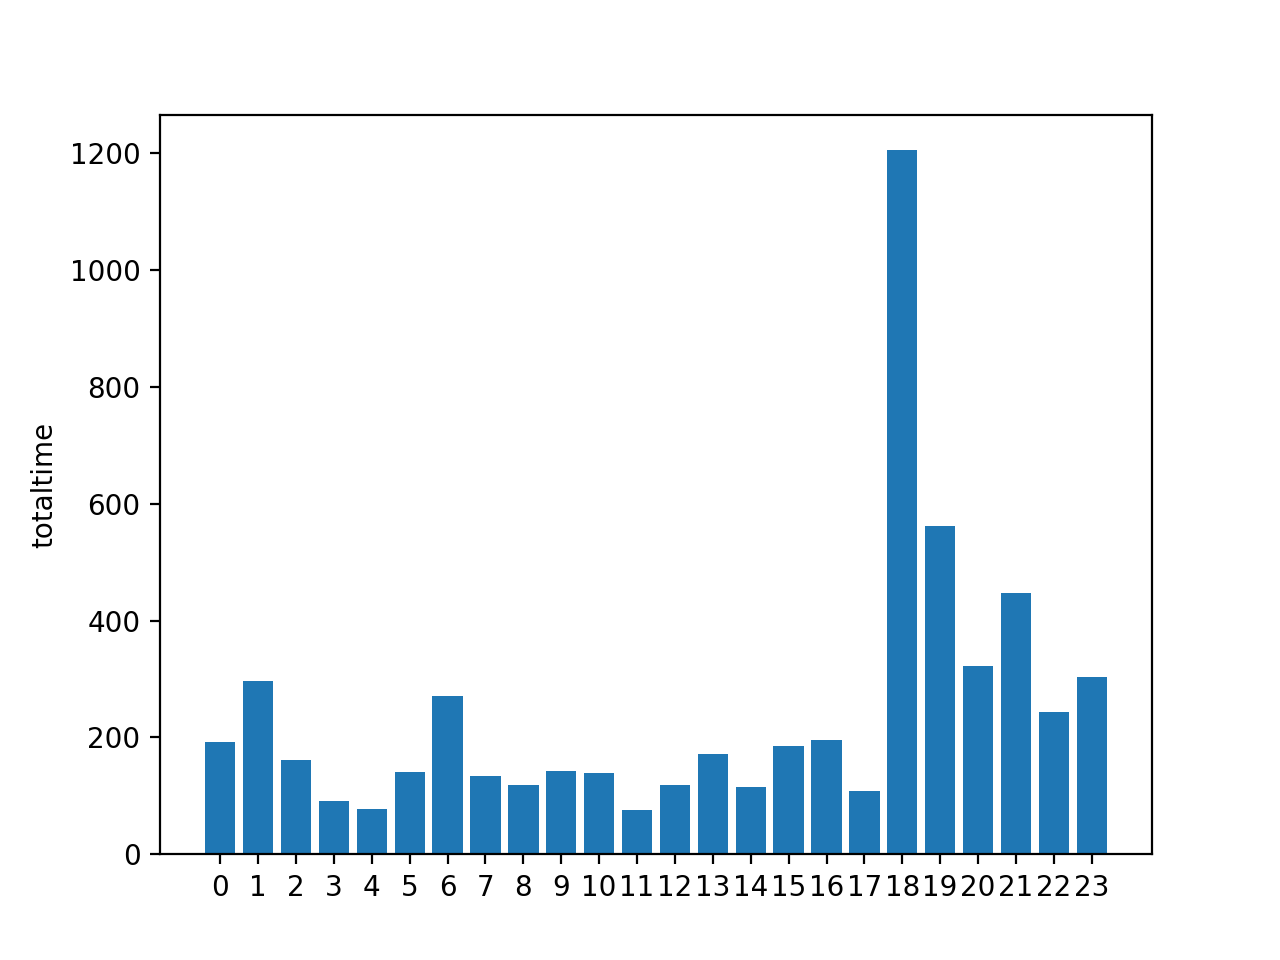
\includegraphics[width=0.7\linewidth]{../../thesis-statisticmethods/statistic_analysis/figures/bar_chart/allParticipants_sorted_Age_Participant_exclude4_notitle}
	\caption{Total time for all participants ordered by age}
	\label{fig:allparticipantssortedageparticipantexclude4notitle}
\end{figure}

The average time spent on the survey was 18 minutes. The two oldest participants used on average 33 minutes, while the rest of the participants spent on average 13 minutes. 

After the pilot test the data was used to test some statistical methods. 


\subsubsection{Statistics result}
First the pilot-test result need to be normality tested. 
As mentioned in \ref{subsec:normaltesting} this thesis will use the Anderson-Darling test. The python library Scipy has an Anderson-Darling test function \citep{TheScipycommunity2017}, this was used to answer the normality test with the Anderson-Darling hypothesis. Testing the total time data form all participants (in total 32 entries) in Anderson-Darling gave a \textit{p-value} of 0.717. The null hypothesis cannot be rejected, then there are two possible cases. One can either accept the null hypothesis or the sample size is not large enough to either accept or reject the null hypothesis \citep{ThePennsylvaniaStateUniversity2017}. An acceptance of the null hypothesis implies that the evidence was insufficient, the result does not necessary accept $H_{0}$, but fails to reject $H_{0}$ \citep{Walpole2012}.  

\begin{framed}{\noindent\centering
\textit{Anderson-Darling test} \\
\textbf{Data:} All participants - total time, 32 entries\\
  \textbf{P-value:} 0.717  \\
    \textit{P-value} > 0.05\\
  \textbf{$H_{0}$:} Accepted, failed to reject \\
  \textit{Anderson-Darling test} \\
  \textbf{Data:} All participants - total time, 32 entries\\
  \textbf{P-value:} 0.717  \\
  \textit{P-value} > 0.05
  \par}
\end{framed}



